\section{Results}
\label{sec:results}

\subsection{Overall Performance}
\label{sec:overall}

\Tabref{tab:overall} summarizes overall performance.
\gptlarge achieves a mean $\tau = 0.948$ with 54.5\% exact-match rate, while \gptsmall achieves $\tau = 0.867$ with 47.0\% exact match.
The difference is statistically significant (Wilcoxon signed-rank $W = 10.5$, $p = 0.008$), confirming that the larger model has more reliable access to the knowledge required for ordering.

\begin{table}[t]
    \centering
    \caption{Overall ordering performance. \gptlarge significantly outperforms \gptsmall across all metrics (Wilcoxon $p = 0.008$). Best results in \textbf{bold}.}
    \label{tab:overall}
    \begin{tabular}{@{}lccc@{}}
        \toprule
        \textbf{Model} & \textbf{Mean $\tau$} & \textbf{Std $\tau$} & \textbf{Exact Match (\%)} \\
        \midrule
        \gptlarge & \textbf{0.948} & \textbf{0.064} & \textbf{54.5} \\
        \gptsmall & 0.867 & 0.190 & 47.0 \\
        \bottomrule
    \end{tabular}
\end{table}

\subsection{Performance by Property Category}
\label{sec:by_category}

\Tabref{tab:category} breaks down performance by property category, and \Figref{fig:category} visualizes the comparison.
Both models achieve perfect scores on syntactic ordering ($\tau = 1.0$).
\gptlarge also achieves $\tau = 1.0$ on well-known factual sequences, while \gptsmall drops to $\tau = 0.884$---notably failing on continent area ($\tau = 0.651$).
Temporal ordering is near-perfect for \gptlarge ($\tau = 0.974$) and strong for \gptsmall ($\tau = 0.926$).
General knowledge and specific factual tasks are harder for both models, with \gptsmall showing particularly high variance.

A Kruskal--Wallis test across categories yields $H = 7.79$, $p = 0.10$ for \gptlarge and $H = 4.17$, $p = 0.38$ for \gptsmall.
The lack of significance at $\alpha = 0.05$ reflects compressed variance (most tasks score above 0.8) rather than true homogeneity---the trends are consistent and interpretable.

\begin{table}[t]
    \centering
    \caption{Mean \kendalltau by property category. Syntactic and well-known sequences are easiest; specific numeric facts are hardest. Best per-category result in \textbf{bold}.}
    \label{tab:category}
    \begin{tabular}{@{}lcc@{}}
        \toprule
        \textbf{Category} & \textbf{\gptlarge $\tau$} & \textbf{\gptsmall $\tau$} \\
        \midrule
        Syntactic & $\mathbf{1.000} \pm 0.000$ & $\mathbf{1.000} \pm 0.000$ \\
        Well-known factual & $\mathbf{1.000} \pm 0.000$ & $0.884 \pm 0.165$ \\
        Temporal & $\mathbf{0.974} \pm 0.045$ & $0.926 \pm 0.054$ \\
        General knowledge & $\mathbf{0.909} \pm 0.049$ & $0.843 \pm 0.164$ \\
        Specific factual & $\mathbf{0.930} \pm 0.075$ & $0.810 \pm 0.256$ \\
        \bottomrule
    \end{tabular}
\end{table}

\begin{figure}[t]
    \centering
    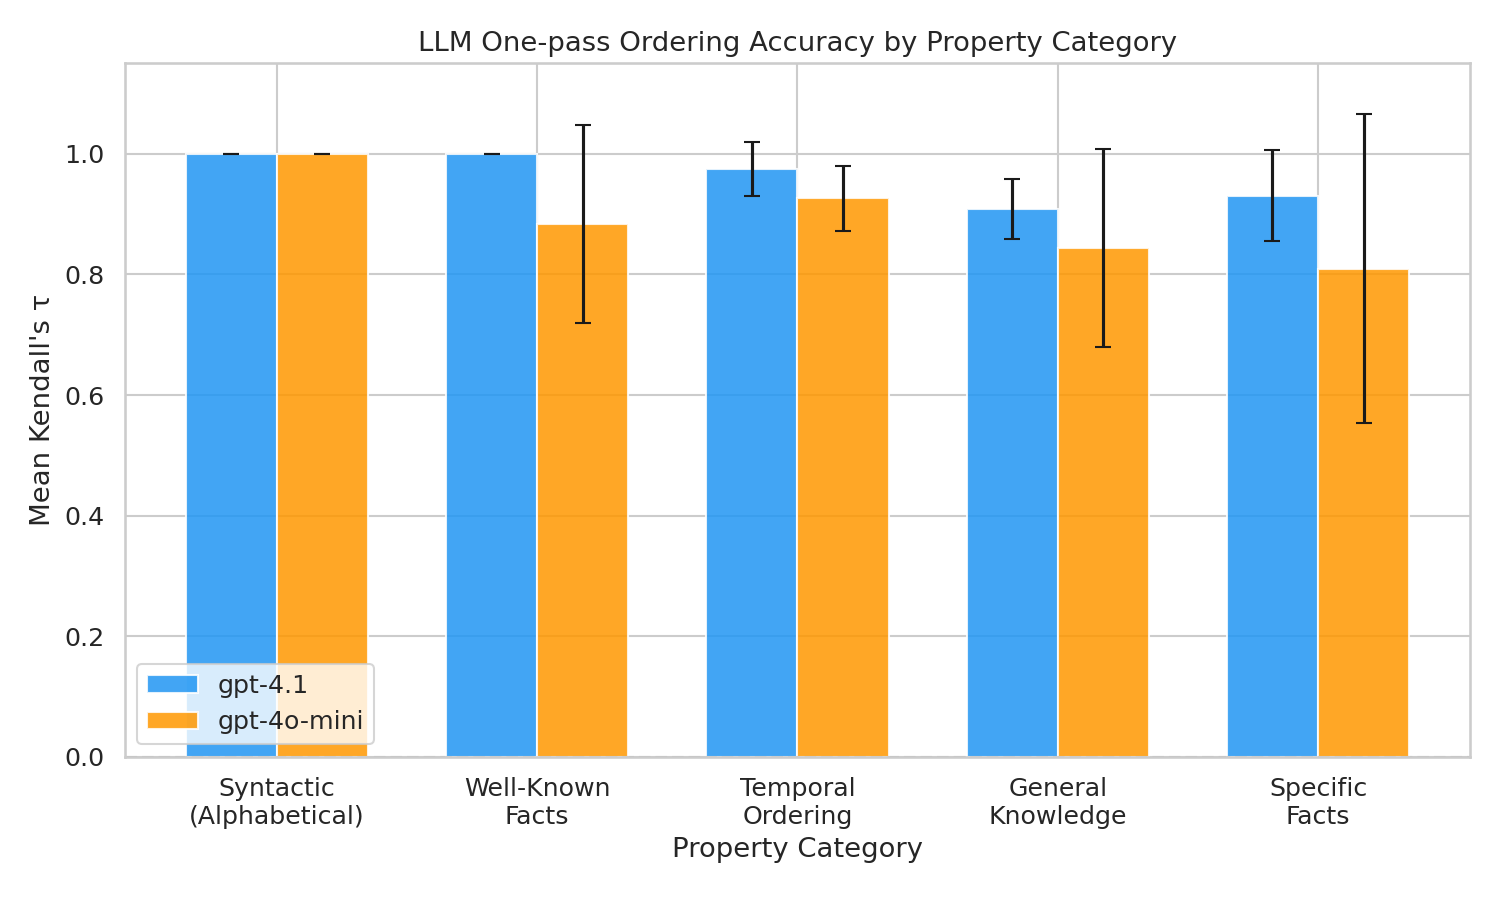
\includegraphics[width=0.95\linewidth]{figures/category_comparison.png}
    \caption{Mean \kendalltau by property category for \gptlarge and \gptsmall. Both models excel at syntactic ordering and struggle most with specific numeric facts, but \gptlarge maintains uniformly high performance while \gptsmall degrades on harder categories.}
    \label{fig:category}
\end{figure}

\subsection{Per-Task Ranking}
\label{sec:per_task}

\Figref{fig:ranking} ranks all 22 tasks by \gptlarge $\tau$ score, and \Figref{fig:heatmap} shows the full task$\times$model heatmap.
Ten tasks achieve perfect scores ($\tau = 1.0$): both alphabetical tasks, all three well-known factual tasks, three of four temporal tasks, and three specific-factual tasks that correspond to well-known educational sequences (element atomic number, color wavelength, Mohs hardness).

The bottom five tasks all involve ordering by continuous numeric properties: city elevation ($\tau = 0.807$), country area ($\tau = 0.822$), city latitude ($\tau = 0.852$), building height ($\tau = 0.867$), and river length ($\tau = 0.881$).
None of these achieves any exact matches for \gptlarge.

\begin{figure}[t]
    \centering
    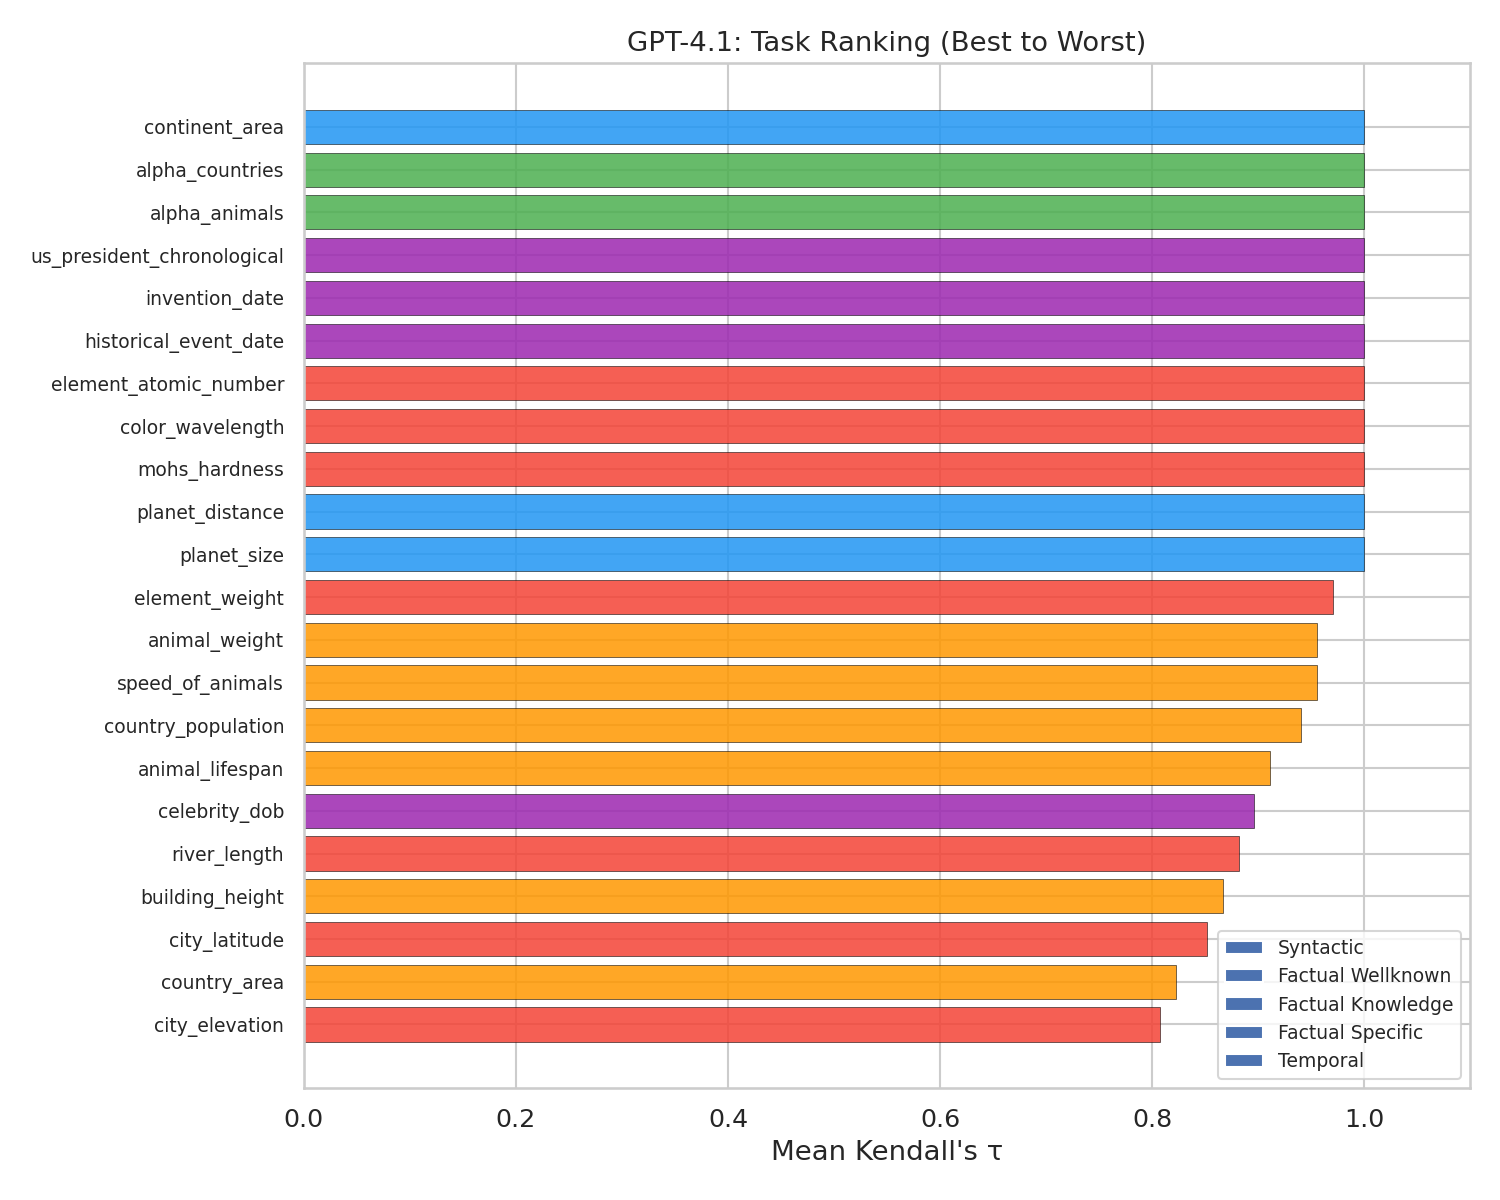
\includegraphics[width=0.95\linewidth]{figures/task_ranking.png}
    \caption{All 22 tasks ranked by \gptlarge \kendalltau. Tasks at the top involve well-known sequences or algorithmic operations; tasks at the bottom require precise numeric recall of independent facts. No bottom-five task achieves a single exact match.}
    \label{fig:ranking}
\end{figure}

\begin{figure}[t]
    \centering
    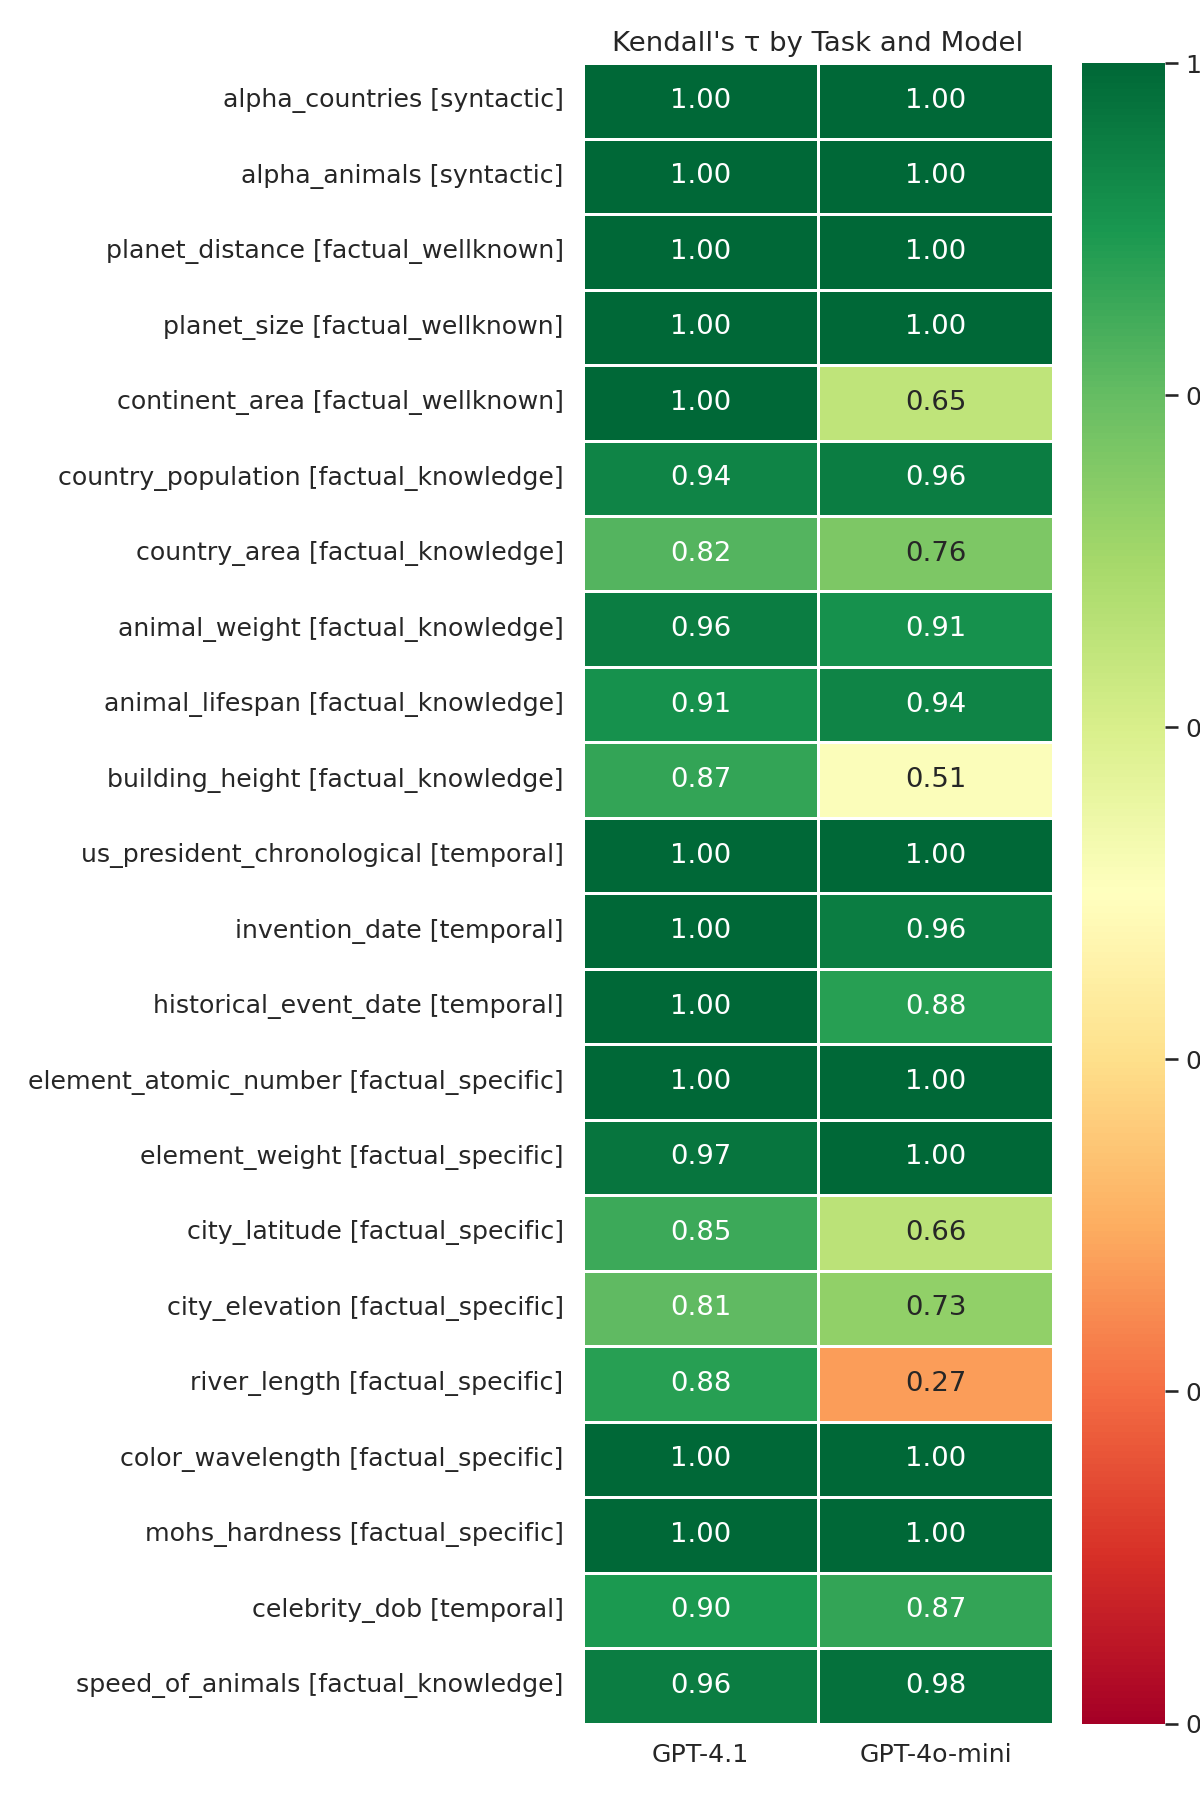
\includegraphics[width=0.95\linewidth]{figures/task_heatmap.png}
    \caption{Heatmap of \kendalltau across all task--model combinations. \gptlarge is uniformly strong (dark), while \gptsmall shows several near-failure tasks (light cells), especially river length ($\tau = 0.274$).}
    \label{fig:heatmap}
\end{figure}

\subsection{Cross-Model Agreement}
\label{sec:agreement}

\Figref{fig:agreement} plots per-task $\tau$ for \gptlarge against \gptsmall.
The cross-model Spearman correlation is $\rho = 0.611$ ($p = 0.003$): the two models largely agree on which properties are easy and which are hard.
This suggests that the property-accessibility hierarchy reflects genuine differences in how knowledge is encoded in language model training data, not idiosyncrasies of a particular model.

The main divergence is in the magnitude of failure.
\gptsmall exhibits catastrophic failures on tasks where \gptlarge merely struggles: river length drops to $\tau = 0.274$ (near random) for \gptsmall versus $\tau = 0.881$ for \gptlarge, and building height drops to $\tau = 0.511$ versus $\tau = 0.867$.

\begin{figure}[t]
    \centering
    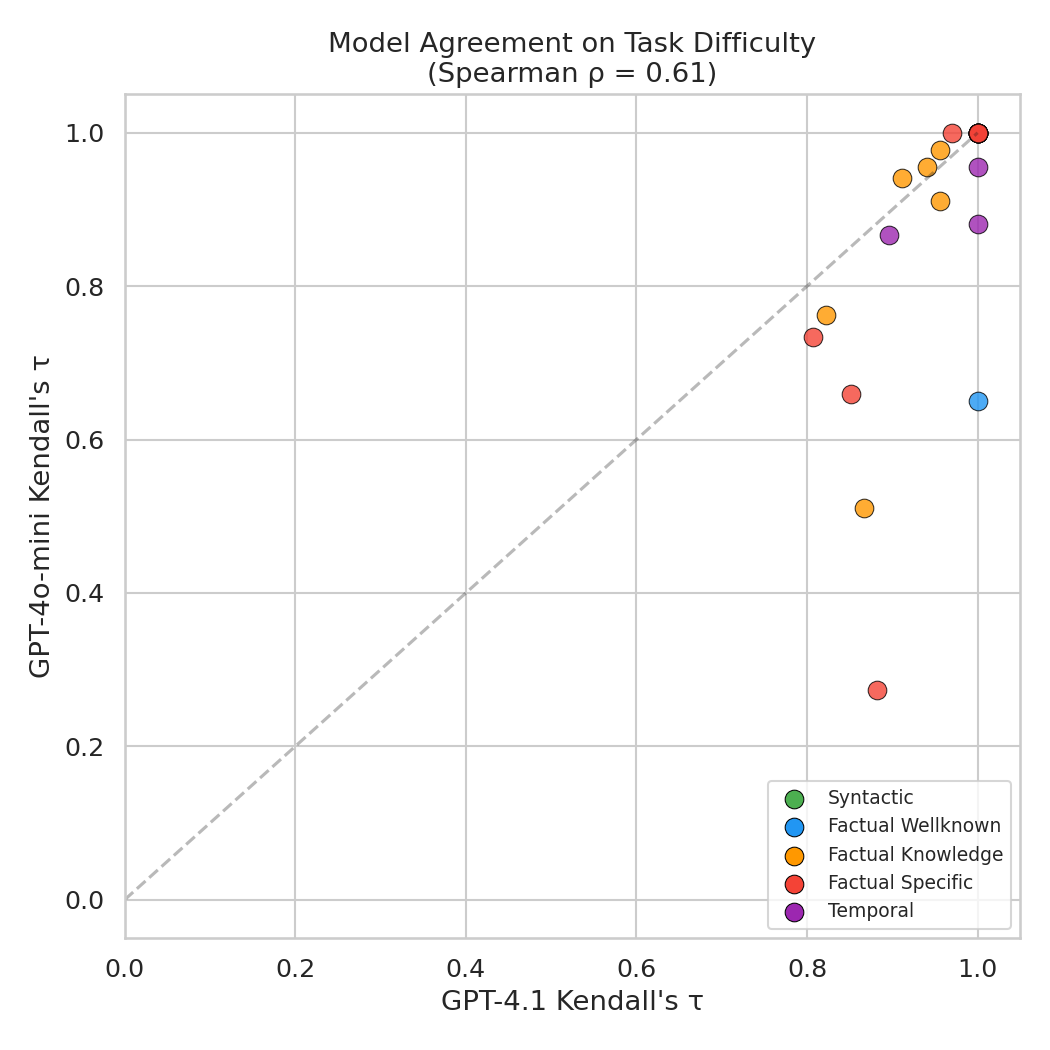
\includegraphics[width=0.7\linewidth]{figures/model_agreement.png}
    \caption{Cross-model agreement. Each point is one task; axes show \kendalltau for \gptlarge ($x$) and \gptsmall ($y$). Spearman $\rho = 0.611$ ($p = 0.003$). Both models agree on the difficulty ranking, but \gptsmall has a longer tail of near-random failures.}
    \label{fig:agreement}
\end{figure}

\subsection{The Property-Accessibility Hierarchy}
\label{sec:hierarchy}

Synthesizing the above results, we identify five levels of property accessibility for LLMs, ordered from easiest to hardest:

\begin{enumerate}[leftmargin=*,itemsep=0pt,topsep=0pt]
    \item \textbf{Algorithmic/syntactic} ($\tau \approx 1.0$): Alphabetical sorting---a mechanical operation on token representations.
    \item \textbf{Famous sequences} ($\tau \approx 1.0$): Planet order, periodic table positions, Mohs scale, color spectrum---memorized as fixed sequences in training data.
    \item \textbf{Historical chronology} ($\tau \approx 0.97$): U.S.\ presidents, inventions, historical events---strong temporal associations in text.
    \item \textbf{Approximate magnitudes} ($\tau \approx 0.93$): Animal weights, speeds, country populations---rough categorical size knowledge.
    \item \textbf{Precise numeric facts} ($\tau \approx 0.83$): City elevations, river lengths, building heights---requires recall of specific independent numbers.
\end{enumerate}

The key insight is that the distinction between easy and hard does not align with the intuitive notion of ``well-known'' versus ``obscure.''
Element atomic numbers and Mohs hardness values are arguably obscure, yet they are perfectly ordered because they form commonly-taught \emph{sequences}.
Conversely, major world rivers and famous buildings are well-known, yet their precise lengths and heights are hard to order because each value must be recalled independently.
